% JC3509 workshop paper template adapted from the CVPR 2025 author kit.
\documentclass[10pt,twocolumn,letterpaper]{article}

\usepackage[pagenumbers]{cvpr}
\input{preamble}

\definecolor{cvprblue}{rgb}{0.21,0.49,0.74}
\usepackage[pagebackref,breaklinks,colorlinks,allcolors=cvprblue]{hyperref}

\def\paperID{JC3509-GroupXX}
\def\confName{CVPR}
\def\confYear{2025}

\title{Using Random Forest and Multi-Layer Perceptron for Adult Income Classification}

\author{
Jinjia Kang (50091025)\\
Aberdeen Institute of Data Science and Artificial Intelligence\\
University of Aberdeen / SCNU\\
{\tt\small 50091025}
\and
Yongdong Li (50091023)\\
Aberdeen Institute of Data Science and Artificial Intelligence\\
University of Aberdeen / SCNU\\
{\tt\small 50091023}
}

\begin{document}
\maketitle
\begin{abstract}
This paper studies adult income prediction as a binary classification problem on the public Adult dataset. The task is to predict whether an individual's annual income exceeds \$50K from 14 demographic and employment-related attributes. We compare two substantially different machine learning methods covered in the module: Random Forest and Multi-Layer Perceptron (MLP). Both models are trained and evaluated under the same preprocessing pipeline, stratified 70/15/15 data split, and validation-based model selection protocol. On the held-out test set, Random Forest achieved higher Accuracy (0.8622), Precision (0.7812), and ROC-AUC (0.9141), while MLP achieved higher Recall (0.6269) and F1-score (0.6765). In practical terms, the MLP recovered more high-income cases, whereas Random Forest made fewer false positive predictions. MLP was also the more efficient method, training faster and requiring far less memory and storage. The main finding is therefore not that one model dominates the other, but that the preferred method depends on deployment priorities: Random Forest is the safer choice when conservative positive predictions and simpler interpretation matter most, while MLP is more attractive when balanced retrieval and low computational cost are more important.
\end{abstract}

\section{Introduction}

Income prediction is a practical classification problem with applications in labour economics, policy analysis, and benefit targeting. It is also a useful machine learning benchmark because errors do not all have the same implication: a model that predicts too many people as high-income behaves very differently from one that misses too many true high-income cases. That makes the task suitable for comparing not only overall accuracy, but also the type of mistakes made by different models.

In this project, we study the Adult income dataset from the UCI Machine Learning Repository~\cite{kohavi1996adult,uciadult}. Our objective is to determine whether a Random Forest classifier~\cite{breiman2001randomforest} or a Multi-Layer Perceptron (MLP)~\cite{rumelhart1986backprop,goodfellow2016deep} is better suited to predicting whether an individual's income exceeds \$50K. This is a meaningful comparison because the dataset is structured and mixed-type, which often suits tree ensembles, but it is still large enough to test whether a neural network can learn competitive decision boundaries after careful preprocessing.

Our study focuses on three practical questions. First, can the task be framed in a clean and reproducible pipeline from data preparation to final evaluation? Second, how differently do a tree ensemble and a neural network behave when trained on the same structured dataset? Third, do their computational costs tell a different story from their predictive scores? These questions shape the comparison carried out in the rest of the paper.

The rest of the paper is organised as follows. Section~\ref{sec:problem_setting} defines the task and dataset. Section~\ref{sec:methodology} presents the compared models. Section~\ref{sec:experimental_setup} describes the experimental protocol, and Section~\ref{sec:results} discusses the quantitative findings.

\section{Problem Setting}
\label{sec:problem_setting}

We address a supervised binary classification problem. Let $\mathbf{x} \in \mathcal{X}$ denote a structured feature vector describing one individual, and let $y \in \{0,1\}$ denote the income label, where $1$ corresponds to annual income greater than \$50K and $0$ otherwise. The goal is to learn a classifier $f(\mathbf{x})$ that predicts the income class for unseen examples.

The Adult dataset contains 48,842 rows with 14 predictive features and one binary income label~\cite{uciadult}. Among the 14 features, 6 are numeric and 8 are categorical. The class distribution is moderately imbalanced: 11,687 positive examples ($>$50K) and 37,155 negative examples ($\leq$50K). The features include age, work class, education, occupation, relationship, sex, capital gain, capital loss, and hours worked per week. This makes the dataset a realistic tabular classification benchmark with mixed data types and non-trivial decision boundaries.

The preprocessing strategy follows the assessment brief. Missing values represented by ``?'' are treated as unavailable observations. Numeric features are imputed with the median, categorical features are imputed with the most frequent category, and categorical variables are transformed through one-hot encoding. Standardization is applied only for the MLP because neural networks are more sensitive to feature scale, whereas tree-based models are generally insensitive to monotonic feature scaling. No target information from the validation or test split is used during preprocessing, which helps avoid data leakage.

This setting is appropriate for the assignment because it uses a public dataset, a clearly defined objective, and a task where both performance and computational trade-offs can be analysed rigorously.

\section{Methodology}
\label{sec:methodology}

\paragraph{Random Forest.}
Random Forest is an ensemble method that averages the outputs of multiple decision trees trained on bootstrapped data subsets~\cite{breiman2001randomforest}. It is a strong baseline for Adult because the data contain mixed numeric and categorical attributes, missing values handled by imputation, and potentially non-linear threshold effects such as changes around age, capital gain, or working hours. Tree ensembles can model such interactions without assuming linear separability and remain comparatively stable when some one-hot encoded columns are sparse or weakly informative. In this project, the search space includes $n\_estimators \in \{200, 500\}$, $max\_depth \in \{\texttt{None}, 20, 40\}$, and $min\_samples\_leaf \in \{1, 5\}$. The best validation configuration was 500 trees with maximum depth 20 and minimum leaf size 1.

\paragraph{Multi-Layer Perceptron.}
The second method is a fully connected neural network trained with back-propagation~\cite{rumelhart1986backprop}. MLPs can learn smooth, high-order decision boundaries after categorical expansion and feature scaling, which makes them a reasonable contrast to tree ensembles even though tabular problems are not always their strongest setting. Here the MLP tests whether a compact neural model can recover competitive performance from the same information while using much less memory at inference time. The explored configurations use hidden layer sizes $(128, 64)$ and $(256, 128)$, with $\alpha \in \{10^{-4}, 10^{-3}\}$, learning rate $\in \{10^{-3}, 5\times10^{-4}\}$, early stopping enabled, and a maximum of 100 training epochs. The best validation configuration used hidden layers $(128,64)$, $\alpha = 0.001$, and learning rate $0.001$.

\paragraph{Why these two methods.}
The assessment requires two methods with substantially different modelling assumptions. Random Forest and MLP satisfy this requirement because one relies on many local decision rules aggregated across trees, while the other learns a shared parametric representation through gradient-based optimisation. This makes the pair suitable for a meaningful comparison of prediction quality, computational cost, and interpretability on the same tabular task. It also avoids a weaker comparison between two closely related variants from the same model family.

\section{Experimental Setup}
\label{sec:experimental_setup}

All experiments use the same stratified train/validation/test split with proportions 70\%/15\%/15\% and random seed 42, resulting in 34,189 training examples, 7,326 validation examples, and 7,327 test examples. The validation set is used for model selection, while the test set is reserved for the final comparison only. This design avoids data leakage and ensures that both methods are evaluated under identical conditions.

The implementation uses Python 3.12.7, \texttt{scikit-learn}, and a Windows 11 environment. The machine reports 31.82 GB of RAM. Model selection is based on validation F1-score, which is appropriate for this task because the Adult dataset is not perfectly balanced and F1-score captures the trade-off between precision and recall. The final reported performance metrics are Accuracy, Precision, Recall, F1-score, and ROC-AUC.

To keep the comparison fair, both methods use the same data split, the same cleaned inputs, and the same validation-driven model-selection rule. We do not apply class re-weighting or task-specific threshold tuning for only one method, because that would confound the comparison. Early stopping is enabled for the MLP to reduce overfitting, while the Random Forest is controlled through the depth and leaf-size search grid. This setup does not make the models identical in capacity, but it does ensure that each model is evaluated under a consistent and defensible protocol.

To complement predictive performance, we also measure practical efficiency. The code records training time, approximate memory growth during training, average inference time per sample, and the size of the serialized model file. These measurements are useful for discussing engineering trade-offs between the two approaches, especially because the assignment requires critical comparison rather than metric reporting alone.

For reproducibility, the repository provides fixed hyperparameter grids, deterministic data splits, and an evaluation script that automatically exports CSV, Markdown, and \LaTeX{} tables. The processor was reported by Python as Intel64 Family 6 Model 183 Stepping 1 on an AMD64 machine profile.

\section{Quantitative Evaluation}
\label{sec:results}

Table~\ref{tab:main_results} reports the final test-set metrics for both models. The exact values are generated automatically by \texttt{src/evaluate.py} and imported directly into the paper. Random Forest achieves the strongest Accuracy (0.8622), Precision (0.7812), and ROC-AUC (0.9141). In contrast, MLP achieves stronger Recall (0.6269) and a slightly better F1-score (0.6765), which was also the model-selection metric.

\IfFileExists{../outputs/tables/main_results_table.tex}{
    \input{../outputs/tables/main_results_table.tex}
}{
    \begin{table}[t]
    \centering
    \caption{Test-set classification metrics for the two compared models.}
    \label{tab:main_results}
    \begin{tabular}{lccccc}
    \toprule
    Model & Acc. & Prec. & Rec. & F1 & ROC-AUC \\
    \midrule
    Random Forest & TBD & TBD & TBD & TBD & TBD \\
    MLP & TBD & TBD & TBD & TBD & TBD \\
    \bottomrule
    \end{tabular}
    \end{table}
}

Table~\ref{tab:complexity_results} summarises the computational trade-offs. MLP is substantially more efficient: it trains in 7.92 seconds compared with 15.65 seconds for Random Forest, uses far less additional memory (1.28 MB vs.\ 175.66 MB), performs much faster inference per sample, and produces a dramatically smaller serialized model.

\IfFileExists{../outputs/tables/complexity_table.tex}{
    \input{../outputs/tables/complexity_table.tex}
}{
    \begin{table}[t]
    \centering
    \caption{Complexity and efficiency comparison on the held-out test set.}
    \label{tab:complexity_results}
    \begin{tabular}{lcccc}
    \toprule
    Model & Train(s) & Infer(ms) & Memory(MB) & Size(MB) \\
    \midrule
    Random Forest & TBD & TBD & TBD & TBD \\
    MLP & TBD & TBD & TBD & TBD \\
    \bottomrule
    \end{tabular}
    \end{table}
}

\begin{figure}[t]
    \centering
    \IfFileExists{../outputs/figures/roc_curve.pdf}{
        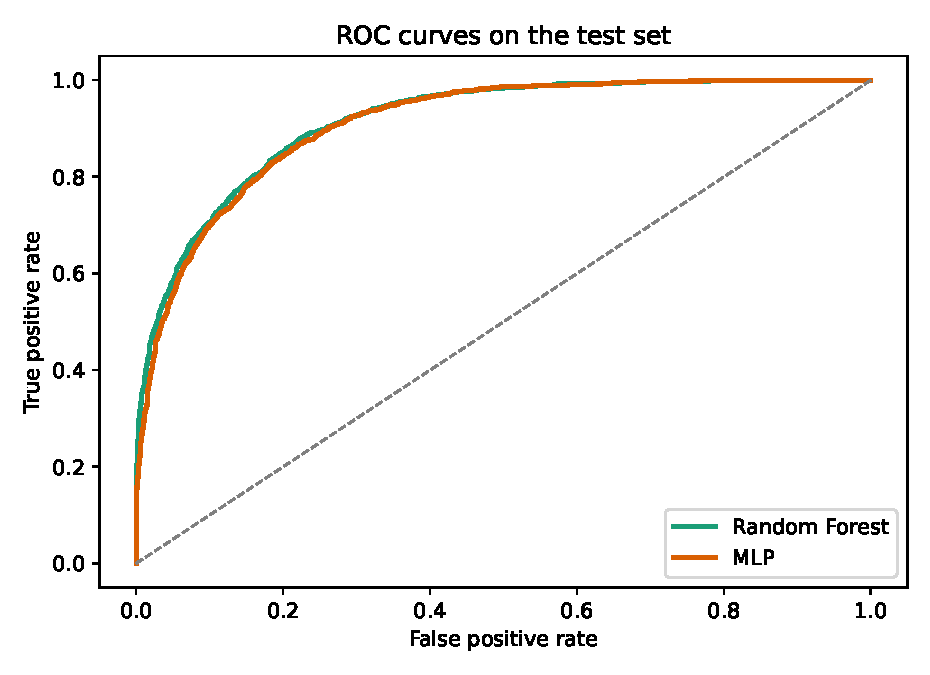
\includegraphics[width=\linewidth]{../outputs/figures/roc_curve.pdf}
    }{
        \fbox{\rule{0pt}{1.65in}\rule{0.95\linewidth}{0pt}}
    }
    \caption{ROC curves for the two models on the test split.}
    \label{fig:roc_curve}
\end{figure}

\begin{figure}[t]
    \centering
    \IfFileExists{../outputs/figures/rf_feature_importance.pdf}{
        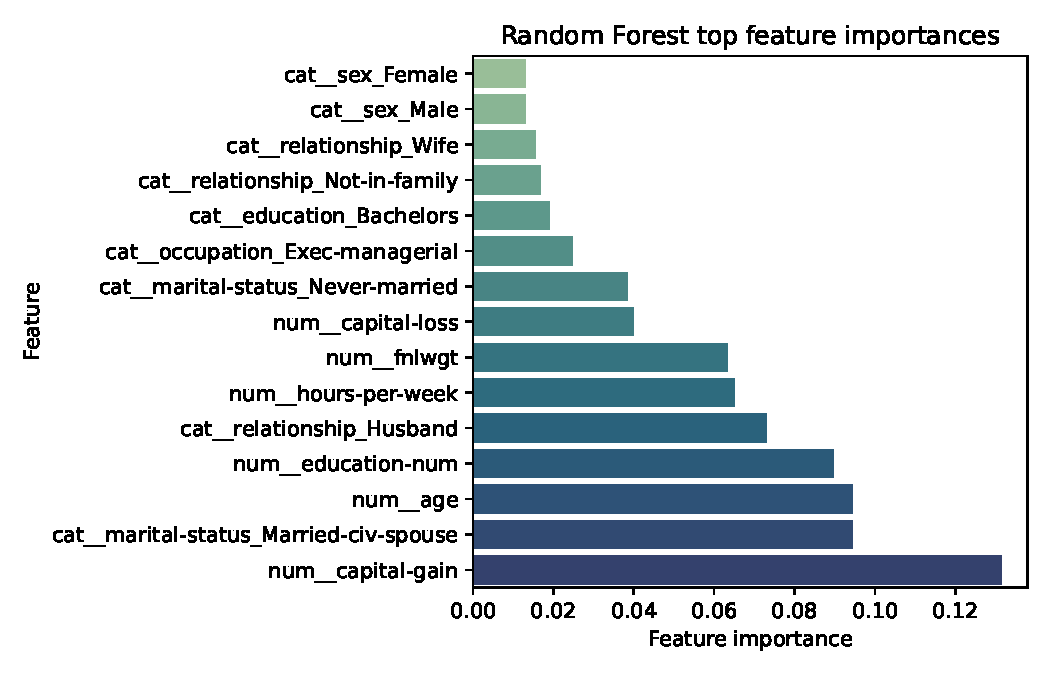
\includegraphics[width=\linewidth]{../outputs/figures/rf_feature_importance.pdf}
    }{
        \fbox{\rule{0pt}{1.65in}\rule{0.95\linewidth}{0pt}}
    }
    \caption{Random Forest feature importance visualisation.}
    \label{fig:rf_importance}
\end{figure}

\paragraph{Discussion.}
The comparison shows that neither model dominates every metric, so the headline result is a trade-off rather than a simple winner. Relative to MLP, Random Forest improves Precision by 4.66 percentage points and ROC-AUC by 0.54 points, but loses 3.82 points of Recall and 0.51 points of F1. In confusion-matrix terms, the MLP identifies 67 additional true high-income cases on the test set, but it also introduces 108 more false positives. This is a useful difference to report because it explains how two models with similar overall scores can behave differently in practice.

The ROC curves in Figure~\ref{fig:roc_curve} show that both models separate the classes well overall, with only a modest gap between them. The main difference is therefore not raw separability, but operating behaviour at the default decision threshold. Random Forest is the more conservative classifier: when it predicts income above \$50K, it is more often correct, but it also leaves more positive cases undiscovered. The MLP behaves in the opposite way, sacrificing some precision to recover more of the minority class.

Figure~\ref{fig:rf_importance} also makes the result easier to interpret. The most influential Random Forest features are capital gain, marital-status indicators, age, education-num, relationship, and hours-per-week. These variables are plausible for the Adult task and align with the intuition that income is associated with accumulated earnings signals, life stage, and labour-market position. At the same time, the importance ranking should not be read as causal evidence; it only indicates which variables helped this model partition the dataset most effectively.

Taken together, the results suggest that MLP is the better default choice when storage, memory use, and balanced retrieval matter most, especially because its F1-score is the strongest while its computational footprint is tiny. Random Forest remains attractive when the user values conservative positive predictions, slightly stronger discrimination, and easier post-hoc explanation of what drove the model's decisions.

\section{Conclusion}

This project compared a Random Forest classifier and a Multi-Layer Perceptron on the Adult income prediction task using a shared preprocessing and evaluation pipeline. The central finding is that model choice changes the type of errors made, not just the headline score. Random Forest achieved higher Accuracy, Precision, and ROC-AUC, while MLP achieved higher Recall and F1-score. In addition, MLP was much faster to train and infer with, used far less memory, and produced a much smaller model file.

For this dataset, MLP is the better overall recommendation if the goal is a compact and efficient classifier that still captures a reasonable share of the positive class. Random Forest remains the stronger option when conservative positive predictions and easier model inspection are more important than footprint. In other words, the better model depends on whether the application penalises false positives or missed positives more heavily.

The main limitations of this study are the restricted hyperparameter search space and the fact that only two model families were compared. In addition, the analysis stays at the level of aggregate predictive performance, so it does not address fairness, calibration, or subgroup-specific behaviour. Natural next steps would therefore include broader tuning, stronger tabular baselines such as gradient boosting, and a more explicit analysis of demographic disparities in model errors.

{
    \small
    \bibliographystyle{ieeenat_fullname}
    \bibliography{refs}
}

\end{document}
